\documentclass[a4paper,11pt]{article}
\usepackage[utf8]{inputenc}
\usepackage[style=ieee]{biblatex}
\usepackage{amsmath, amssymb, amsthm}
\usepackage{hyperref}
\usepackage[capitalize]{cleveref}
\usepackage{graphicx}
\usepackage{caption}
\usepackage{booktabs}

\newcommand{\IM}{i} % change i with j for electrical engineering
\newcommand{\EXP}[1]{e^{#1}} % comment for \exp instead of e^{}
% \newcommand{\EXP}[1]{\exp\left(#1\right)} % and uncomment for \exp

\title{Title}
\author{Name Surname}
\date{\today}
\bibliography{bibliography}
\hypersetup{
    colorlinks=true,
    linkcolor=red,
    urlcolor=blue,
    citecolor=green,
}

\begin{document}
\maketitle

\section{Dummy Section}
This is a dummy section with an inline equation \(F = ma\), a set of
aligned mathematical identities in~\cref{eq:general,eq:special}, and
a book reference of~\autocite{knuth1997art}.
\begin{align}
	\EXP{\IM\theta}  & = \cos(\theta)+\IM\sin(\theta)~\label{eq:general} \\
	1 + \EXP{\IM\pi} & = 0~\label{eq:special}
\end{align}
In addition, an image and a table are also provided in~\cref{fig:space}
and~\cref{tab:mytable}, respectively.
\begin{figure}[h]
	\centering{}
	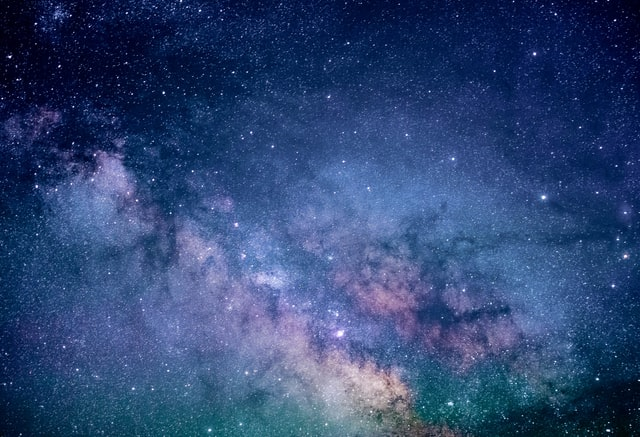
\includegraphics[width=0.5\linewidth]{images/space.jpg}
	\caption{Stock Image by Jeremy Thomas
		(\href{https://bit.ly/3AUuKM7}{link})}\label{fig:space}
\end{figure}
\begin{table}[h]
	\centering{}
	\caption{My Table}\label{tab:mytable}
	\begin{tabular}{ccc}\toprule
		\textbf{Column A} & \textbf{Column B} & \textbf{Column C} \\ \midrule
		1                 & 2                 & 3                 \\
		4                 & 5                 & 6                 \\
		\bottomrule
	\end{tabular}
\end{table}


\printbibliography{}
\end{document}
